\chapter{Felhasznált technológiák}

\thispagestyle{fancy}
\pagestyle{fancy}

Munkám során törekedtem arra, hogy a felhasznált technológiákat lehetőleg minimalizáljam. 
Figyelembe vettem továbbá azt is, hogy nyílt forráskódú, és multiplatform eszközöket válasszak. Ezen döntések lehetővé tették számomra a kellő flexibilitást, és elősegítették a munkámat.
\section{Godot Engine}
A Godot \cite{Introduc48:online} egy nyílt forráskódú, ingyenesen elérhető játékmotor és fejlesztői környezet, amelyet a játékok, interaktív tartalmak és egyéb multimédiás alkalmazások létrehozására terveztek. A motorot Juan Linietsky, Ariel Manzur és George Marques alapította 2014-ben \cite{TheEvolu53:online}, és azóta folyamatos fejlesztés alatt áll, számos kiadott verzióval és fejlesztői közösséggel.

A Godot kiemelkedik sokoldalúsága és könnyűsége miatt. Az egyik legfontosabb jellemzője az integrált fejlesztői környezet (IDE), amely segítségével a fejlesztők egyetlen alkalmazásban végezhetik el a játékterv készítését, a kódolást, a grafika létrehozását és a játéktesztek futtatását. Az IDE rendelkezik számos funkcióval, mint például kódszerkesztő, jelenet szerkesztő, animációkészítő, fizikai motor, hangkezelő, és még sok más, amelyek egyszerűsítik és gyorsítják a fejlesztési folyamatot.

A Godot támogatja a kettő dimenziós (2D) és a három dimenziós (3D) játékfejlesztést is, és számos előre elkészített funkciót és sablont kínál mindkét típushoz. A motor különösen erős a vizuális effektek, az animációk és a szkriptelés terén, és lehetővé teszi a fejlesztők számára, hogy rugalmasan alkalmazzák saját ötleteiket és terveiket a játék készítése során.
 
A Godot-t széles körben használják különböző projektekben, beleértve az indie játékokat, oktatási alkalmazásokat, interaktív médiaalkotásokat. A motor aktív és elkötelezett fejlesztői közösséggel rendelkezik, amely folyamatosan hozzájárul az új funkciók, javítások és dokumentációk fejlesztéséhez.

Átgondoltam a további lehetőségeimet is.
Választhattam volna az Unreal Engine-t \cite{unrealengine}, amely egy fejlett, 3D játékok fejlesztésére specializálódott játékmotor. 
Azonban a rendszerkövetelményei túl magasak voltak számomra. A másik opcióm a Unity \cite{UnityRea46:online} volt.
Összehasonlítottam a Unity-t  a Godot-al és arra jutottam, hogy a Godot GDScript nyelve sokkal könnyebben használható, mint a Unity C++ nyelve, így végül a Godot mellett döntöttem. 

\section{GDScript}
A GDScript\cite{GDScript64:online} a Godot Engine saját szkript nyelve, melyet játékfejlesztéshez terveztek, könnyen tanulható és használható nyelv. 

A GDScript egy dinamikus típusú script nyelv, ami által egyszerűbb és rugalmasabb kódolási stílust tesz lehetővé.

Támogatja az objektumorientált programozás alapvető elveit, mint például az osztályok, az öröklődés és a polimorfizmus. 
Emellett rendelkezik számos beépített funkcióval és osztállyal, melyek jelentősen megkönnyítik a játékprogram készítését.

\section{itch.io}
Az itch.io \cite{Introduc10:online} (kisbetűs írásmóddal) egy web platform, ahol a felhasználók, és fejlesztők indie videojátékokat, szerepjátékokat, játékelemeket, képregényeket, és zeneszámokat oszthatnak meg, árusíthatnak és tölthetnek le. A weboldalt Leaf Corcoran indította 2013 márciusában, és 2023 áprilisi állapot szerint több mint 700,000 termék található rajta.

Az itch.io támogatja, hogy HTML5-be kiexportált és feltöltött játékokkal a böngészőből bárki játszhasson egy gombnyomással.

\section{CloudFlair}
Cloudflare \cite{WhyCloud84:online} egy biztonságos és megbízható megoldás, amely lehetővé teszi, hogy a helyi szervereket nyilvános domain név alatt érjük el, anélkül, hogy közvetlenül kinyitnánk a tűzfalat. Ez jelentősen növeli a biztonságot, mivel a szerver közvetlenül nem lesz kitéve az internet veszélyeinek, miközben a szolgáltatás könnyen elérhető marad.

\section{Node.js}
A Node.js \cite{Nodejs—R76:online} egy nyílt forráskódú, platformfüggetlen JavaScript futtatókörnyezet, amely a V8 JavaScript motort használja. A Node.js lehetővé teszi a fejlesztők számára, hogy szerveroldali alkalmazásokat készítsenek JavaScript nyelven. Egyedülálló eseményvezérelt, nem-blokkoló I/O modellt alkalmaz, amely rendkívül hatékony és alkalmas adatintenzív valós idejű alkalmazások fejlesztésére. A Node.js ökoszisztémája rendkívül gazdag, köszönhetően a npm (Node Package Manager) csomagkezelőnek, amely több százezer ingyenesen elérhető modul közül válogathat.

\section{Docker}
A Docker \cite{DockerAc99:online} egy nyílt forráskódú platform, amely lehetővé teszi az alkalmazások konténerizálását, skálázhatóságát és hordozhatóságát. A Docker konténerek könnyű, elszigetelt környezeteket biztosítanak, amelyekben az alkalmazások futtathatók. Ezek a konténerek tartalmazzák az összes szükséges függőséget és konfigurációt, így az alkalmazások bármilyen környezetben, változtatás nélkül futtathatók. A Docker egyszerűvé teszi az alkalmazások telepítését és frissítését, miközben minimalizálja az „egy gépen működik, de másikon nem” problémákat. A Docker Compose \cite{DockerCo66:online} lehetőséget biztosít több konténer egyidejű kezelésére és orkestrációjára, ami különösen hasznos komplex alkalmazások esetében.

\section{Express}
Az Express.js \cite{ExpressN40:online}, vagy egyszerűen Express, egy minimalista és rugalmas Node.js webalkalmazás keretrendszer, amely gazdag funkcionalitással rendelkezik webalkalmazások és API-k fejlesztéséhez. Az Express leegyszerűsíti a szerver felépítését és konfigurálását, és számos köztes réteget (middleware) kínál, amelyek megkönnyítik a különböző feladatok kezelését, mint például az adatfeldolgozás, az autentikáció, a session kezelés, és a fájlkezelés. Az Express előnye, hogy könnyen bővíthető és integrálható más modulokkal és eszközökkel, ami gyors és hatékony fejlesztést tesz lehetővé.

\section{Python 3}
A Python 3 \cite{AboutPyt99:online} egy magas szintű, dinamikusan típusos programozási nyelv, amely 2008-ban jelent meg. Egyszerű és olvasható szintaxisával, valamint széleskörű könyvtáraival gyorsan népszerűvé vált. Támogatja az objektumorientált programozást és különböző alkalmazási területekhez, például webfejlesztéshez, adatfeldolgozáshoz és gépi tanuláshoz kínál eszközöket. Keresztplatformos működése miatt könnyen használható különböző operációs rendszereken, és aktív közössége folyamatosan bővíti és fejleszti.

\section{TensorFlow}
A TensorFlow \cite{tensorflow2015-whitepaper} egy nyílt forráskódú szoftverkönyvtár gépi tanuláshoz és mesterséges intelligenciához.
Eredetileg a Google Brain csapat fejlesztette, és mára az egyik legnépszerűbb és legszélesebb körben használt keretrendszer a gépi tanulási modellek fejlesztéséhez és futtatásához.
A TensorFlow rugalmas és moduláris architektúrája lehetővé teszi a különböző típusú neurális hálózatok könnyű fejlesztését és tréningezését. Különféle eszközöket és könyvtárakat kínál, amelyek támogatják a mély tanulási, természetes nyelvfeldolgozási és kép-felismerési feladatokat.
A TensorFlow-t széles körben használják kutatók és ipari szakemberek egyaránt a mesterséges intelligencia és gépi tanulás területén.

\section{Keras}
A Keras \cite{chollet2015keras} egy könnyen használható API, amely a TensorFlow alapjaira épül, és leegyszerűsíti a mélytanulási modellek fejlesztését. Segítségével gyorsan és egyszerűen lehet modelleket létrehozni, tesztelni és tanítani, ami különösen hasznos prototípusok készítésekor és kísérletezéskor. Kihasználja a TensorFlow erejét és rugalmasságát, miközben felhasználóbarát marad.

\section{SHA256}
Az SHA-256 \cite{rfc4634} egy hash-függvény, amely bármilyen méretű adatot 256 bites (32 bájtos) kóddá alakít. Széles körben használják biztonsági alkalmazásokban, például digitális aláírásokban és adatintegritás ellenőrzésére. Az SHA-256 az SHA-2 család tagja, és erős kriptográfiai tulajdonságai miatt nehéz visszafejteni.

\section{Flask}
A Flask \cite{grinberg2018flask} egy könnyű és rugalmas webkeretrendszer Python nyelvhez, amely lehetővé teszi gyors webalkalmazások fejlesztését. 2010-ben indult, és mikrokeretrendszerként minimalista alapokkal rendelkezik, de könnyen bővíthető különböző modulokkal. Fő jellemzői közé tartozik az egyszerűség, rugalmasság és a RESTful API-k támogatása. Ideális választás egyszerű webalkalmazásokhoz, prototípusokhoz és nagyobb projektekhez is a megfelelő bővítmények segítségével.

\section{draw.io}
A draw.io \cite{Aboutdra31:online} egy ingyenesen használható, webalapú diagramkészítő eszköz, amely lehetővé teszi a felhasználók számára, hogy könnyedén készítsenek és osszanak meg különböző diagramokat, folyamatábrákat, és vázlatokat. Ezzel készítettem több ábrámat is. 

\section{LaTeX}
A LaTeX egy nagy teljesítményű dokumentum-előkészítő rendszer, amely különösen népszerű tudományos és műszaki területeken; a szakdolgozatomat is ebben írtam, és az ábráim egy részét is ezzel a rendszerrel készítettem, mivel kiváló tipográfiai minőséget biztosít és hatékonyan kezeli a bonyolult elrendezéseket.

\section{ChatGPT}
A ChatGPT \cite{Introduc55:online} az OpenMI által fejlesztett mesterséges intelligencia alapú nyelvi modell, amely természetes nyelven folytat beszélgetéseket. Képes megérteni a felhasználói kérdéseket, és releváns válaszokat generálni széleskörű tudásbázisából. Interaktív és kontextusérzékeny, így alkalmazható információkeresésre, kreatív írásra és sok más feladatra. Folyamatosan fejlődik, hogy javítsa a felhasználói élményt.

A projektemben a ChatGPT-t felhasználtam, hogy a szakdolgozatomat stilisztikailag kijavítsa, a formázás szempontjából felgyorsítsa az írás folyamatát. Használtam a mesterséges intelligencia tanító kódjának leírásához, mint iránymutató, valamint a webapplikáció elkészítésében is a segítségét kértem. Ezeken kívűl mint fordító is használtam, hogy az angol dokumentációkat magyarra fordítsam. 
\begin{figure}[h]
    \center
    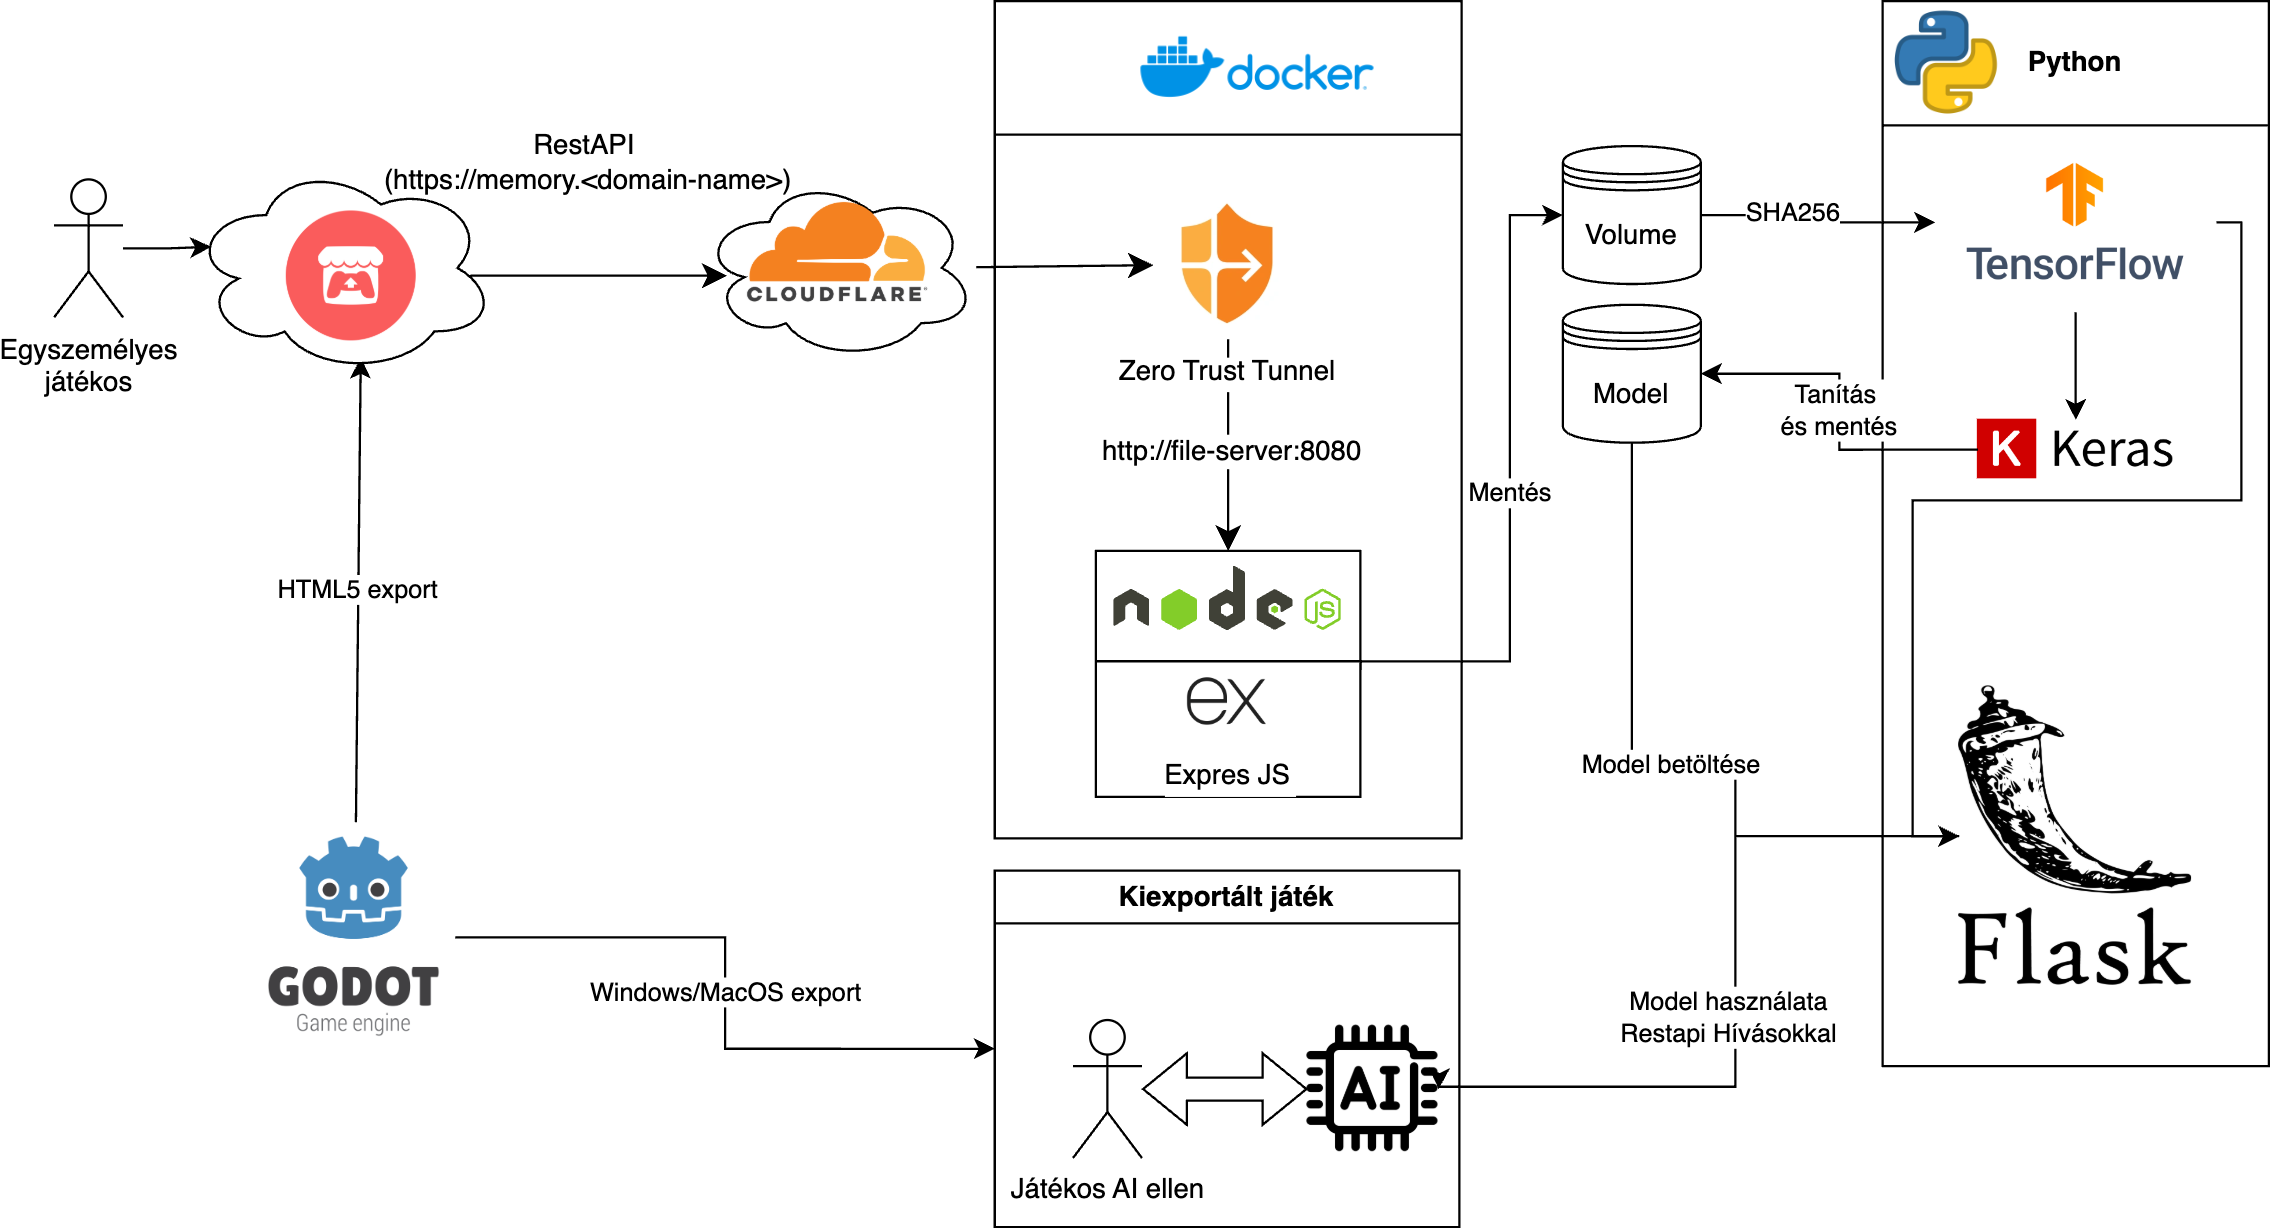
\includegraphics[width=\textwidth]{img/fullfolyamat.png}
    \caption{A felhasznált technológiák kapcsolata}
    \label{img:technology}
\end{figure}